\section{Introdução}

%\subsection{Motivação}

O interesse na área da robótica se dá pela multi-disciplinaridade do tema, que abrange um espectro de conhecimentos que vai desde mecânica estrutural até a aplicação de teorias de controle sofisticadas. A área ainda se estende por eletrônica, elétrica, computação e até mesmo psicologia. Assim, considera-se que esta área é bastante adequada a um trabalho de conclusão de um curso igualmente abrangente, que é a Engenharia de Controle e Automação.

Em aplicações industriais, a maioria dos robôs utilizados são manipuladores, que realizam tarefas repetitivas -- como soldagem ou montagem de peças -- com precisão e rapidez adequados a cada aplicação. Estes robôs, no entanto, são em geral fixos, e daí surge o estudo da robótica móvel: como um robô pode se mover sem supervisão humana e interagir com o mundo real? \citep{siegwart2011introduction} Além do interesse acadêmico, existe um significativo interesse comercial, visto que o mercado de robôs móveis, que estava em torno de 4,5 bilhões de dólares americanos em 2014, tende a duplicar até 2020 \citep{marketsmarkets}.

\begin{figure}[h]
  \centering
  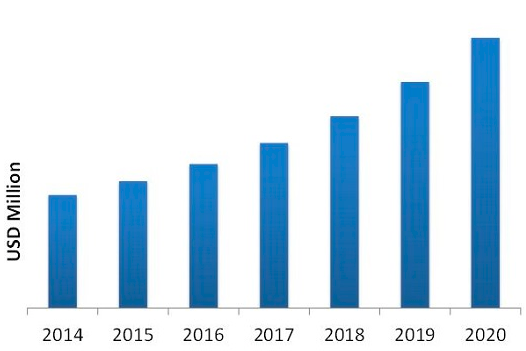
\includegraphics[width = 0.5\textwidth]{imagens/markets}
  \caption{Projeção de crescimento do mercado de robótica móvel até 2020.}
  \label{fig:markets}
  \source{\citet{marketsmarkets}}
\end{figure}

Segundo \citet{lynch2017modern}, robôs móveis são divididos em não-holonômicos e omnidirecionais, com diferenças significativas em planejamento de trajetória, controle e modelagem dos dois tipos de robô. Diante da natureza do presente trabalho de conclusão de curso, o escopo foi definido no âmbito dos robôs omnidirecionais, que se destacam pela habilidade de realizar transporte de cargas pequenas em espaços confinados -- como corredores de hospital e depósitos de armazenamento que buscam o aumento da capacidade sem perder agilidade logística nem aumentar o espaço necessário nas instalações. Academicamente, o controle de rodas omnidirecionais apresenta diversos problemas atrativos, vários dos quais serão descritos ao longo do presente trabalho. O desenvolvimento de uma plataforma robótica omnidirecional holonômica se torna útil para futuras aplicações em diversas áreas de investigação em robótica, controle e automação.

%\subsection{Descrição do Trabalho}

O presente trabalho consiste no desenvolvimento (tanto teórico quanto experimental) de uma plataforma robótica que possa se movimentar de maneira autônoma em qualquer direção do plano sem necessidade de reorientação -- apresentando holonomicidade. Após uma avaliação na bibliografia sobre os tipos de robôs factíveis de serem construídos no tempo previsto e com os recursos financeiros disponíveis, optou-se pela configuração descrita na sequência. A plataforma considerada mais adequada utiliza 3 \emph{omniwheels}, cada uma acionada por um motor elétrico dedicado, conforme o modelo mostrado na Figura \ref{fig:tomr_ritter}. Como as rodas são montadas de maneira fixa no chassi, este tipo de robô ainda oferece a vantagem de ser construído com uma estrutura mecânica mais simples, como mencionado por \citet{siciliano2016springer}. As rodas omnidirecionais utilizadas podem ser vistas em detalhes na Figura \ref{fig:omniwheel}. O sistema de movimentação é controlado por software processado em um computador embarcado a partir dos sinais fornecidos por sensores inerciais e de odometria.

\begin{figure}[h]
  \centering
  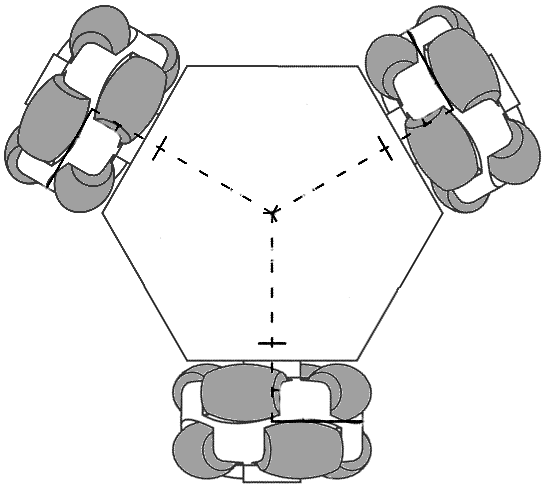
\includegraphics[width = 0.45\textwidth]{imagens/tomr_ritter_mod}
  \caption{Diagrama de um robô móvel com três rodas omnidirecionais.}
  \label{fig:tomr_ritter}
  \source{Adaptado de \citet{ritter2016modelagem}}
\end{figure}

\begin{figure}[h]
  \centering
  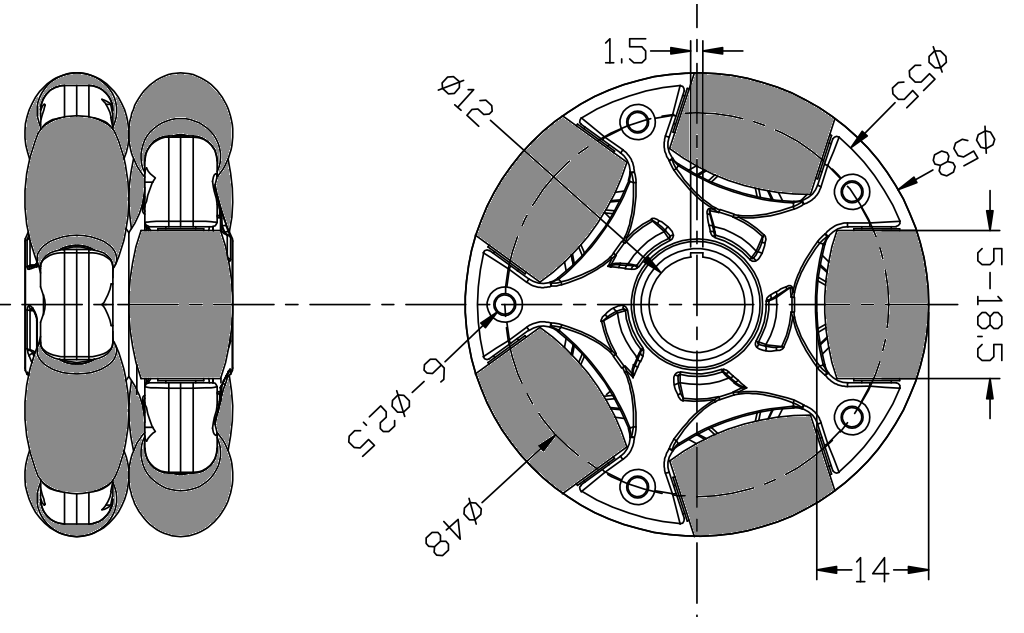
\includegraphics[width = 0.45\textwidth]{imagens/omniwheel}
  \caption{Desenho de uma roda omnidirecional.}
  \label{fig:omniwheel}
  \source{Adaptado de \citet{omniwheel}}
\end{figure}

%\subsection{Objetivos}

Este trabalho tem como \textbf{objetivo geral} projetar, construir, colocar em operação e testar uma plataforma robótica omnidirecional de baixo custo, mas com características semelhantes às dos sistemas comerciais. Para atingir esse objetivo, se devem alcançar os seguintes \textbf{objetivos específicos}:

\begin{itemize}
  \item{Modelagem do robô;} %especificar se é cinemática ou dinâmica
  \item{Especificação e construção de um protótipo;}
  \item{Implantação de um algoritmo de controle;} % eu tinha colocado implementação, mas perondi pediu implantação
  \item{Implantação de instrumentação;}
  \item{Análise de uma proposta preliminar de algoritmo de odometria;}
  \item{Realizar experimentos de seguimento de trajetórias e analisar os resultados obtidos.}
\end{itemize}

%\subsection{Organização do Trabalho}

O trabalho está organizado da seguinte maneira:
\begin{itemize}
  \item{Na \hyperref[sec:revbib]{Seção 2}, é apresentada a revisão bibliográfica, versando sobre robótica móvel, técnicas de controle utilizadas na área e um breve resumo sobre métodos de localização, além de uma exposição dos trabalhos mais recentes envolvendo robôs omnidirecionais;} %colocar planejamento de trajetória e hardware tbm??
  \item{Na \hyperref[sec:montagem]{Seção 3}, foca-se na especificação do hardware, estrutura mecânica e montagem do protótipo;}
  \item{Na \hyperref[sec:teorico]{Seção 4}, é apresentado o desenvolvimento teórico da modelagem do robô e dos algoritmos de controle e localização;}
  \item{Na \hyperref[sec:software]{Seção 5} são implementados os algoritmos descritos na seção anterior;}
  \item{Na \hyperref[sec:experimental]{Seção 6}, é descrito um experimento para avaliar o desempenho do robô projetado e são apresentadas as análises e discussões sobre os resultados dos experimentos, a conclusão sobre o trabalho como um todo e algumas propostas para futuros trabalhos.}
\end{itemize}

Além do descrito, o trabalho ainda contém o \hyperref[sec:custo]{Apêndice A}, da descrição dos custos do projeto.

%
%Além do descrito, o trabalho ainda contém os seguintes apêndices:
%\begin{itemize}
%  \item{\hyperref[sec:custo]{Apêndice A}, da descrição dos custos do projeto;}
%  \item{\hyperref[sec:loop]{Apêndice B}, com o código fonte da função executada periodicamente para o controle;}
%  \item{\hyperref[sec:draw]{Apêndice C}, que mostra as dimensões da plataforma projetada.}
%\end{itemize}
